\section{Model}
\label{sec:arrhythmias:model}

\subsection{Problem Formulation}

The ECG arrhythmia detection task is a sequence-to-sequence task which takes as
input an ECG signal $X=[x_1,.. x_T]$, and outputs a sequence of labels $Y=[y_1,
... y_U]$, such that each $y_u$ can take on one of 12 different rhythm
classes. Each output label corresponds to a segment of the input. Together the
output labels cover the full sequence.

For a single example in the training set, we optimize the cross-entropy
objective function
\[
 \mathcal{L}(X, Y) = \frac{1}{U} \sum_{u=1}^U \log p(y_u \mid X)
\]
where $p(\cdot)$ is the probability that the network assigns to the $u$-th
output taking on the value $y_u$.

\subsection{Model Architecture and Training}

We use a convolutional neural network for the sequence-to-sequence learning
task. The high-level architecture of the network is shown in
Figure~\ref{fig:arrhythmias:net}. The network takes as input a time-series of
raw ECG signal, and outputs a sequence of label predictions. The 30 second long
ECG signal is sampled at 200Hz, and the model outputs a new prediction once
every 256 samples. After careful architectur search, arrive at a model which is
33 layers of convolution followed by a fully connected layer and a softmax. 

\begin{figure}
\centering
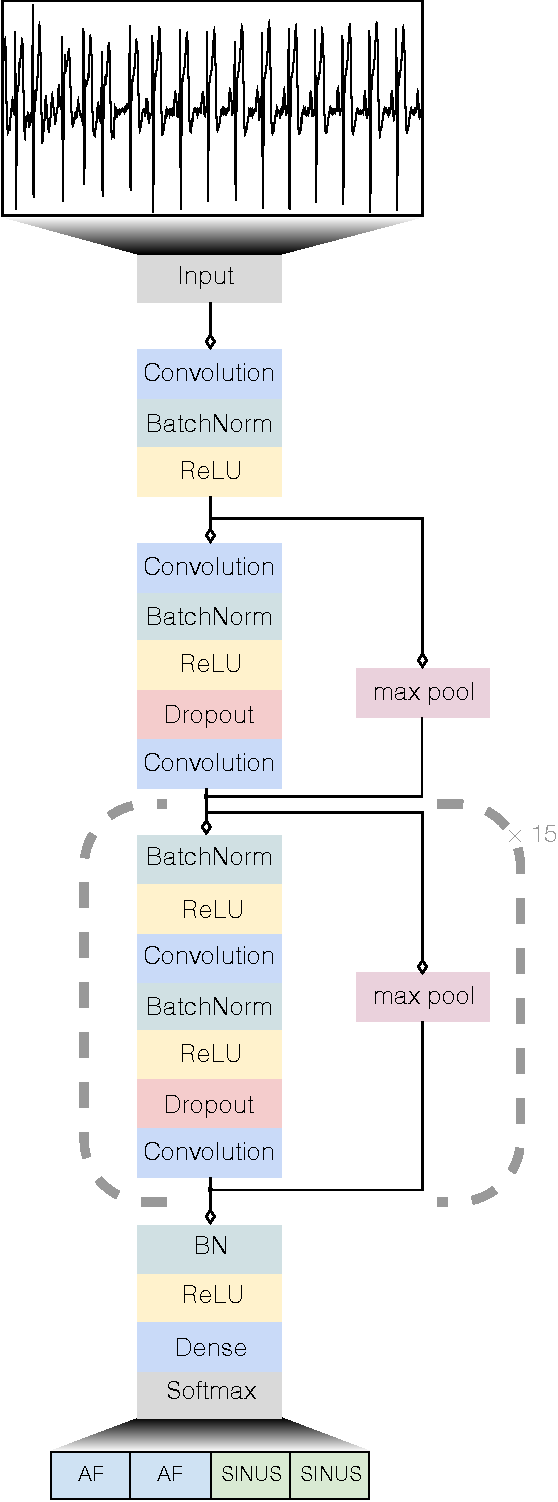
\includegraphics[width=0.4\textwidth]{arrhythmias/figures/ecg_network_full.pdf}
\caption{The architecture of the deep neural network consists of 33
         convolutional layers followed by a fully-connected layer and
         a softmax layer.}
\label{fig:arrhythmias:net}
\end{figure}

In order to make the optimization of such a network tractable, we employ
shortcut connections in a similar manner to those found in the Residual Network
architecture~\cite{he2016identity}. The shortcut connections between
neural-network layers optimize training by allowing information to propagate
well in very deep neural networks. Before the input is fed into the network, it
is normalized using a robust normalization strategy. The network consists of 16
residual blocks with 2 convolutional layers per block. The convolutional layers
all have a filter length of 16 and have 64$k$ filters, where $k$ starts out as
1 and is incremented every 4-th residual block. Every alternate residual block
subsamples its inputs by a factor of 2, thus the original input is ultimately
subsampled by a factor of $2^8$. When a residual block subsamples the input,
the corresponding shortcut connections also subsample their input using a Max
Pooling operation with the same subsample factor. 

Before each convolutional layer we apply Batch
Normalization~\cite{ioffe2015batch} and a rectified linear activation, adopting
the pre-activation block design~\cite{he2016deep}. The first and last layers of
the network are special-cased due to this pre-activation block structure. We
also apply Dropout~\cite{srivastava2014dropout} between the convolutional
layers and after the non-linearity. The final fully connected layer and softmax
activation produce a distribution over the 12 output classes for each
time-step.

We train the networks from scratch, initializing the weights of the
convolutional layers as in~\cite{he2015delving}. We use the
Adam~\cite{kingma2014adam} optimizer with the default parameters and reduce the
learning rate by a factor of 10 when the validation loss stops improving. We
save the best model as evaluated on the validation set during the optimization
process.
